% !TeX spellcheck = en_GB
\documentclass[a4paper, 10pt]{article}

\usepackage{fontspec}
\usepackage{amsmath, amssymb}
\usepackage{multicol}
\usepackage{color}
\usepackage{colortbl}
\usepackage[dvipsnames]{xcolor}
\usepackage{logicproof}
\usepackage{tikz}
\defaultfontfeatures{Mapping=tex-text,Scale=MatchLowercase}
\setmainfont{Ubuntu Light}

\title{Discrete Mathematics}
\author{Max Kasperowski}

\begin{document}
\maketitle
\tableofcontents

\newpage
\section{Logic}

\subsection[Propositional Logic]{Propositional Logic{\large ---Zeroth Order Logic}}
In propositional logic, propositions are denoted by letters (\(p, q\)) and are formed by connecting other propositions using logical connectives. Propositions can either be true (\(T\)) or false (\(F\)).
\paragraph{Logical Connectives}
The logical connectives listed below are the basic connectives available in propositional logic in order of their precedence. Below are the truthtables corresponding to each of the connectives.
\begin{enumerate}
    \item \( \neg \), not
    \item \( \land \), and, \( \bigwedge\limits_{i=1}^n p_i \)
    \item \( \lor \), or, \( \bigvee\limits_{i=1}^n p_i \)
    \item \( \rightarrow ,\Rightarrow \), implies (only if) defined as: \( p\rightarrow q \equiv \neg p\lor q \)
    \item \( \leftrightarrow ,\Leftrightarrow \), is equivalent to (if and only if, iff) defined as: \(p\leftrightarrow q \equiv (p\rightarrow q)\land (q\rightarrow p) \)
\end{enumerate}

\begin{multicols}{3}
\paragraph{Negation}\mbox{}\\
\begin{tabular}{@{ }c | c@{ }@{ }c}
p & \( \neg \) & p\\
\hline
T & \textcolor{ForestGreen}{F} & T\\
F & \textcolor{ForestGreen}{T} & F\\
\end{tabular}
\paragraph{Logical And}\mbox{}\\
\begin{tabular}{@{ }c@{ }@{ }c | c@{ }@{ }c@{ }@{ }c@{ }@{ }c@{ }@{ }c}
p & q &  & p & \( \land\) & q & \\
\hline
T & T &  & T & \textcolor{ForestGreen}{T} & T & \\
T & F &  & T & \textcolor{ForestGreen}{F} & F & \\
F & T &  & F & \textcolor{ForestGreen}{F} & T & \\
F & F &  & F & \textcolor{ForestGreen}{F} & F & \\
\end{tabular}
\paragraph{Logical Or}\mbox{}\\
\begin{tabular}{@{ }c@{ }@{ }c | c@{ }@{ }c@{ }@{ }c@{ }@{ }c@{ }@{ }c}
p & q &  & p & \( \lor \) & q & \\
\hline
T & T &  & T & \textcolor{ForestGreen}{T} & T & \\
T & F &  & T & \textcolor{ForestGreen}{T} & F & \\
F & T &  & F & \textcolor{ForestGreen}{T} & T & \\
F & F &  & F & \textcolor{ForestGreen}{F} & F & \\
\end{tabular}
\paragraph{Implication}\mbox{}\\
\begin{tabular}{@{ }c@{ }@{ }c | c@{ }@{ }c@{ }@{ }c@{ }@{ }c@{ }@{ }c}
p & q &  & p & \(\rightarrow\) & q & \\
\hline
T & T &  & T & \textcolor{ForestGreen}{T} & T & \\
T & F &  & T & \textcolor{ForestGreen}{F} & F & \\
F & T &  & F & \textcolor{ForestGreen}{T} & T & \\
F & F &  & F & \textcolor{ForestGreen}{T} & F & \\
\end{tabular}
\paragraph{Equivalence}\mbox{}\\
\begin{tabular}{@{ }c@{ }@{ }c | c@{ }@{ }c@{ }@{ }c@{ }@{ }c@{ }@{ }c}
p & q &  & p & \(\leftrightarrow\) & q & \\
\hline
T & T &  & T & \textcolor{ForestGreen}{T} & T & \\
T & F &  & T & \textcolor{ForestGreen}{F} & F & \\
F & T &  & F & \textcolor{ForestGreen}{F} & T & \\
F & F &  & F & \textcolor{ForestGreen}{T} & F & \\
\end{tabular}
\end{multicols}
\subsubsection{Definitions}
\paragraph{Converse, Contrapositive, Inverse}
When given the proposition \( p\rightarrow q \), \( q\rightarrow p \) is its converse, \( \neg q\rightarrow \neg p \) is its contrapositive and \( \neg p\rightarrow \neg q \) is its inverse. The contrapositive is equivalent to the original proposition and the converse and inverse are also equivalent.

\paragraph{Tautology}
A proposition that is always true (\(p\lor\neg p\)).

\paragraph{Contradiction}
A proposition that is always false (\(p\land\neg p\)).

\paragraph{Contingency}
A proposition that is neither a tautology nor a contradiction.

\paragraph{Logical Equivalence}
\(p\) and \(q\) are logically equivalent if \(p\leftrightarrow q\) is a tautology. The notation for equivalence is typically \(\equiv\).
\newpage
\subsubsection{Properties}
\begin{multicols}{2}
    \subparagraph{De Morgan's Laws}
    \[ \neg(p\lor q) \equiv \neg p \land \neg q \]
    \[ \neg(p\land q) \equiv \neg p \lor \neg q \]

    \subparagraph{Identity Laws}
    \[ p \lor F \equiv p \]
    \[ p \land T \equiv p \]

    \subparagraph{Domination Laws}
    \[ p \lor T \equiv T \]
    \[ p \land F \equiv F \]

    \subparagraph{Idempotent Laws}
    \[ p \lor p \equiv p\]
    \[p \land p \equiv p\]

    \subparagraph{Negation Laws}
    \[ p \lor \neg p \equiv T \]
    \[ p \land \neg p \equiv F \]

    \subparagraph{Commutative Laws}
    \[ p \lor q \equiv q \lor p \]
    \[ p \land q \equiv q \land p\]

    \subparagraph{Associative Laws}
    \[ (p \lor q)\lor r \equiv p\lor(q\lor r) \]
    \[ (p \land q)\land r \equiv p\land(q\land r) \]

    \subparagraph{Distributive Laws}
    \[ p\lor (q \land r) \equiv (p\lor q) \land (p\lor r) \]
    \[ p\land (q\lor r) \equiv (p\land q)\lor(p\land r) \]

    \subparagraph{Absorption Laws}
    \[ p \lor (p\land q) \equiv p \]
    \[ p \land (p\lor q) \equiv p \]
\end{multicols}

\subsubsection{Equivalence Proof}
This is an example of how to perform an equivalence proof. The aim is to show that \( \neg(p\lor (\neg p \land q)) \) is logically equivalent to \( \neg p\land \neg q \). We can prove this by forming a series of logical equivalences.
\begin{align*}
    \textcolor{ForestGreen}{\neg (p\lor(\neg p\land q))} &\equiv \neg p \land \neg(\neg p\land q) & \text{2\textsuperscript{nd} De Morgan's law}\\
    \neg p \land \neg(\neg p\land q) &\equiv \neg p \land (p\lor\neg q) & \text{1\textsuperscript{st} De Morgan's law} \\
    \neg p \land (p\lor\neg q) &\equiv (\neg p \land p)\lor(\neg p\land \neg q) & \text{Associative law} \\
    (\neg p \land p)\lor(\neg p\land \neg q) &\equiv F \lor (\neg p \land \neg q) & \text{Negation law} \\
    F \lor (\neg p \land \neg q) &\equiv \textcolor{ForestGreen}{\neg p \land \neg q} & \text{Identity law}
\end{align*}

\newpage
\subsection[Predicate Logic]{Predicate Logic {\large ---First Order Logic}}
Predicate logic uses quantified variables over non-logical objects and allows the use of sentences that contain variables. This allows a generalisation of propositions for a set of variables from a domain.

\subsubsection{Definitions}
\paragraph{Predicates}
A predicate is a generalisation of propositions when the variable \(x\) is replaced by a specific element from its domain. \(P(x)\) becomes a proposition. When no other domain is specified the domain is \(U\).

\paragraph{Quantifiers}
Quantifiers are used to express that a proposition is true for all elements of the domain and that there exists some element in the domain for which it is true. They also have the highest precedence among the logical operators.
\begin{align*}
    \text{Universal quantifier\quad\quad\quad\quad} & \forall xP(x) & P(x)\text{ is true for every \(x\) in \(U\)} \\
    \text{Existential quantifier\quad\quad\quad\quad} & \exists xP(x) & P(x)\text{ is true for some \(x\) in \(U\)}
\end{align*}

\subsubsection{Properties}
\paragraph{Uniqueness Quantifier}
The uniqueness quantifier is a commonly used quantifier to express that there is only one \(x\) for which \(P(x)\) is true. It is usually written as \(\exists !\) or \(\exists_1\).
\[\exists_1xP(x)\equiv\exists x(P(x)\land\forall y(P(y)\rightarrow y=x))\]
\paragraph{De Morgan's Laws}
De Morgan's laws for quantifiers state that \(P(x)\) is not true for all \(x\) if and only if there exists an \(x\) for which \(P(x)\) is false and furthermore that if \(P(x)\) is false for all \(x\) if and only if there does not exist an \(x\) for which \(P(x)\) is true.
\begin{align*}
    \neg\forall x P(x) &\equiv \exists x\neg P(x)\\
    \forall x\neg P(x) &\equiv \neg\exists x P(x)
\end{align*}

\newpage
\subsection{Logical Proofs}
Using logical inference it is possible to build an argument given a set of premises to reach a logical conclusion. An argument is valid if truth of all premises \(p_i\) implies that the conclusion \(q\) is also true.
\[\left(\bigwedge_{i=1}^n p_i\right)\rightarrow q \equiv T\]

\subsubsection{Rules of Inference}
\begin{multicols}{3}
\paragraph{Modus Ponens}\mbox{}\\
\begin{tabular}{c@{\,}l@{}}
                & \(p\rightarrow q\) \\
                & \(p\) \\\cline{2-2}
\(\therefore\)  & \(q\)
\end{tabular}

\paragraph{Modus Tollens}\mbox{}\\
\begin{tabular}{c@{\,}l@{}}
                & \(p\rightarrow q\) \\
                & \(\neg q\) \\\cline{2-2}
\(\therefore\)  & \(\neg p\)
\end{tabular}

\paragraph{Hypothetical Syllogism}\mbox{}\\
\begin{tabular}{c@{\,}l@{}}
                & \(p\rightarrow q\) \\
                & \(q\rightarrow r\) \\\cline{2-2}
\(\therefore\)  & \(p\rightarrow r\)
\end{tabular}

\paragraph{Disjunctive Syllogism}\mbox{}\\
\begin{tabular}{c@{\,}l@{}}
                & \(p\lor q\) \\
                & \(\neg p\) \\\cline{2-2}
\(\therefore\)  & \(q\)
\end{tabular}

\paragraph{Addition}\mbox{}\\
\begin{tabular}{c@{\,}l@{}}
                & \(p\) \\\cline{2-2}
\(\therefore\)  & \(p\lor q\)
\end{tabular}

\paragraph{Simplification}\mbox{}\\
\begin{tabular}{c@{\,}l@{}}
                & \(p\land q\) \\\cline{2-2}
\(\therefore\)  & \(p\)
\end{tabular}
\begin{tabular}{c@{\,}l@{}}
                & \(p\land q\) \\\cline{2-2}
\(\therefore\)  & \(q\)
\end{tabular}

\paragraph{Conjunction}\mbox{}\\
\begin{tabular}{c@{\,}l@{}}
                & \(p\) \\
                & \(q\) \\\cline{2-2}
\(\therefore\)  & \(p\land q\)
\end{tabular}

\paragraph{Resolution}\mbox{}\\
\begin{tabular}{c@{\,}l@{}}
                & \(\neg p\lor r\) \\
                & \(p\lor q\) \\\cline{2-2}
\(\therefore\)  & \(q\lor r\)
\end{tabular}

\paragraph{Universal Instantiation}\mbox{}\\
\begin{tabular}{c@{\,}l@{}}
                & \(\forall xP(x)\) \\\cline{2-2}
\(\therefore\)  & \(P(c)\)
\end{tabular}

\paragraph{Universal Generalisation}\mbox{}\\
\begin{tabular}{c@{\,}l@{}}
                & \(P(c)\) for an arbitrary \(c\) \\\cline{2-2}
\(\therefore\)  & \(\forall xP(x)\)
\end{tabular}

\paragraph{Existential Instantiation}\mbox{}\\
\begin{tabular}{c@{\,}l@{}}
                & \(\exists xP(x)\) \\\cline{2-2}
\(\therefore\)  & \(P(c)\) for some element \(c\)
\end{tabular}

\paragraph{Existential Generalisation}\mbox{}\\
\begin{tabular}{c@{\,}l@{}}
                & \(P(c)\) for some element \(c\) \\\cline{2-2}
\(\therefore\)  & \(\exists xP(x)\)
\end{tabular}

\paragraph{Universal Modus Ponens}
\begin{tabular}{c@{\,}l@{}}
                & \(\forall x(P(x)\rightarrow Q(x))\) \\
                & \(P(a)\) for a particular element \(a\) \\\cline{2-2}
\(\therefore\)  & \(Q(a)\)
\end{tabular}

\end{multicols}

\subsubsection{Inference Proof}
All men are mortal. Socrates is a man. Prove that Socrates is mortal.

\(P(x)\equiv T\) means that \(x\) is a person. \(M(x)\equiv T\) means that \(x\) is mortal. \(s\) is the particular element Socrates.

\begin{logicproof}{0}
    \forall x P(x)\rightarrow M(x) & premise \\
    P(s) & premise \\
    P(s)\rightarrow M(s) & UI (1) \\
    M(s) & Modus Ponens, (2) \& (3)
\end{logicproof}

\newpage
\section{Set Theory}
A set is a collection of distinct elements without duplicates and the order of elements is unimportant.
\subsection{Definitions}
\paragraph{Containment}
\( a \in A \) denotes that \(a\) is an element of the set \(A\), whereas \( a \notin A \) denotes that \(a\) is not contained in \(A\). A set may contain other sets.

\subsubsection{Describing Sets}
\paragraph{Roster Method}
List all elements contained in the set. \( S = \{a, b, c, d\} \) is equivalent to both \( S = \{d, c, a, b\} \) and also \( S = \{a, a, b, c, d, d\} \). When the pattern is clear, (\ldots) may be used as in \( S = \{a, b, c, \ldots, z\} \).

\paragraph{Set-Builder Method}
Specify the proposition that all members must satisfy. \( S = \{x|P(x)\} \) denotes that all elements \(x\) in \(S\) must satisfy the proposition \(P(x)\).

\paragraph{Interval Notation}
The elements in a set can be constrained by an open or closed interval. \( [a, b] = \{x|a\leq x\leq b\} \) represents the closed interval between \(a\) and \(b\). \( (a, b) = \{x|a<x<b\} \) represents the open interval between \(a\) and \(b\). Additionally combinations like \( [a, b) \) and \( (a, b] \) are possible.

\subsubsection{Special Sets}
\paragraph{Universal Set}
The universal set, denoted by \(U\), contains everything currently under consideration.

\paragraph{Empty Set}
The empty set is the set that contains no elements. It is denoted by \(\varnothing\). It is important to note that \(\varnothing = \{\}\), but \( \varnothing \neq \{\varnothing\} \). A set containing the empty set is not the equal to the empty set.

\paragraph{Singleton}
A singleton is a set containing exactly one element.

\subsubsection{Set Equality}
Two sets are equal if they contain the same elements. If \(A\) and \(B\) are sets then their equality is denoted as \(A = B\).
\[ \forall x(x\in A \equiv x\in B)\rightarrow A=B \].

\newpage
\subsubsection{Subsets}
Set \(A\) is a subset of \(B\) if all elements in \(A\) are also in \(B\). This relation is denoted as \(A\subseteq B\).
\[\forall x(x\in A\rightarrow x\in B)\equiv A\subseteq B\]
Every set is always a subset of itself and the empty set \(\varnothing\) is a subset of every other set.
\paragraph{Proper Subset}
When \(A\subseteq B\), but \(A\neq B\) then \(A\) is a proper subset of \(B\), which is denoted as \(A\subset B\).
\[\forall x (x\in A\rightarrow x\in B)\land \exists x(x\in B\land x\notin A)\equiv A\subset B\].

\subsubsection{Set Cardinality}
For finite sets the set cardinality describes the number of distinct elements in a set. It is denoted as \(|S|\). The cardinality of the empty set is zero (\(|\varnothing| = 0\)). If \(A\) is the set containing all the letters of the english alphabet, then \(|A| = 26\).

\subsubsection{Power Sets}
The set of all subsets of a set \(A\) is called the power set of \(A\) and is denoted as \(\mathcal{P}(A)\). If \(|A| = n\), then \(|\mathcal{P}(A)| = 2^n\). For example, given the set \(A = {a, b}\) we get the power set \(\mathcal{P}(A) = \{\varnothing, \{a\}, \{b\}, \{a,b\}\}\).

\subsection{Tuples}
Tuples are a collection of ordered elements. An \(n\)-tuple is written as \((a_1, a_2, a_3,\ldots,a_n).\) Two \(n\)-tuples are equal if and only if all of their corresponding elements are equal.
\[(a,b) = (c,d)\equiv (a=c) \land (b=d)\]
A subset \(R\) of \(A\times B\) is called a relation from the set \(A\) to the set \(B\).

\subsubsection{Cartesian Product}
The cartesian product \(A\times B\) is the set of ordered pairs \((a,b)\) where \(a\in A\) and \(b\in B\).
\[A\times B = \{(a,b)|a\in A \land b\in B\}\]
The cartesian product of \(n\) sets is the set of tuples containing all possible combinations of elements as tuples.
\[ A_1\times A_2\times\ldots\times A_n = \{(a_1, a_2,\ldots, a_n)|a_i\in A_i \text{ for } i=1, 2,\ldots,n\} \]
The cardinality of the cartesian product is equal to the product of the cardinalities of the individual sets.
\[|A_1\times A_2\times\ldots\times A_n| = \prod_{i=1}^n|A_i| \]

\newpage
\subsection{Operations}
The set operators are based on boolean algebra and are analogous to the operators in propositional calculus. There must always be a universal set \(U\) and all sets are assumed to be a subset of \(U\).

\begin{multicols}{2}
\paragraph{Union}\mbox{}\\
The union of \(A\) and \(B\) is the set that contains those elements that are contained in \(A\), \(B\) or in both.
\[ A\cup B = \{x|x\in A \lor x\in B\} \]
\begin{center}
    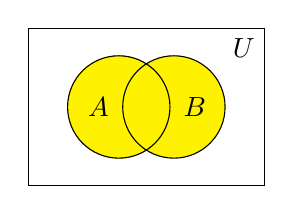
\begin{tikzpicture}
    \draw (0,0) --(0,2) --(3,2) --(3,0) --(0,0);
    \node [left] at (3,1.75){\(U\)};
    \draw [yellow, fill=yellow] (1.15, 1) circle [radius=0.65];
    \draw [fill=yellow] (1.85, 1) circle [radius=0.65];
    \draw (1.15, 1) circle [radius=0.65];
    \node [left] at (1.15,1){\(A\)};
    \node [right] at (1.85, 1){\(B\)};
    \end{tikzpicture}
\end{center}

\paragraph{Intersection}\mbox{}\\
The intersection of \(A\) and \(B\) is the set that contains those elements that are contained in both \(A\) and \(B\).
\[ A\cap B = \{x|x\in A \land x\in B\} \]
\begin{center}
    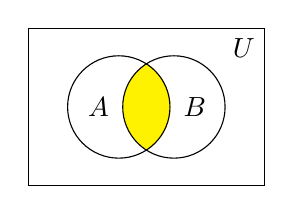
\begin{tikzpicture}
    \draw (0,0) --(0,2) --(3,2) --(3,0) --(0,0);
    \node [left] at (3,1.75){\(U\)};

    \begin{scope}
        \clip (1.85, 1) circle [radius=0.65];
        \draw [yellow, fill=yellow](1.15, 1) circle [radius=0.65];
    \end{scope}
    \draw (1.15, 1) circle [radius=0.65];
    \draw (1.85, 1) circle [radius=0.65];
    \node [left] at (1.15,1){\(A\)};
    \node [right] at (1.85, 1){\(B\)};
    \end{tikzpicture}
\end{center}

\paragraph{Complement}\mbox{}\\
The complement of the set \(A\) contains all the elements in \(U\) that are not in \(A\). It is equivalent to \(U-A\).
\[ \bar{A} = \{x\in U|x\notin A\} \]
\begin{center}
    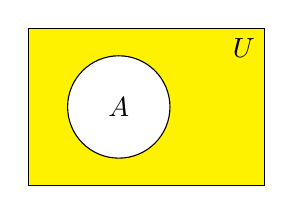
\begin{tikzpicture}
    \draw [fill=yellow](0,0) --(0,2) --(3,2) --(3,0) --(0,0);
    \node [left] at (3,1.75){\(U\)};
    \draw [fill=white](1.15, 1) circle [radius=0.65];
    \node at (1.15,1){\(A\)};
    \end{tikzpicture}
\end{center}

\paragraph{Difference}\mbox{}\\
The difference \(A-B\) is the set that contains all the elements in \(A\) but not in \(B\). It is the union of \(A\) with the complement of \(B\).
\[ A-B = \{x|x\in A \land x\notin B\} = A\cap \bar{B} \]
\begin{center}
    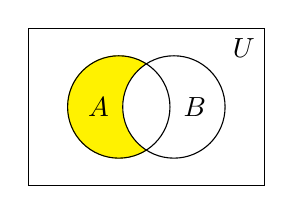
\begin{tikzpicture}
    \draw (0,0) --(0,2) --(3,2) --(3,0) --(0,0);
    \node [left] at (3,1.75){\(U\)};
    \draw [yellow, fill=yellow](1.15, 1) circle [radius=0.65];
    \draw [fill=white] (1.85, 1) circle [radius=0.65];
    \draw (1.15, 1) circle [radius=0.65];
    \node [left] at (1.15,1){\(A\)};
    \node [right] at (1.85, 1){\(B\)};
    \end{tikzpicture}
\end{center}
\end{multicols}
\paragraph{Symmetric Difference}\mbox{}\\
The symmetric difference is equivalent to a logical exclusive or meaning that the symmetric difference between \(A\) and \(B\) contains the elements that are in \(A\) or in \(B\), but not those that are in both \(A\) and \(B\).
\[ A\oplus B = (A-B)\cup(B-A) \]
\begin{center}
    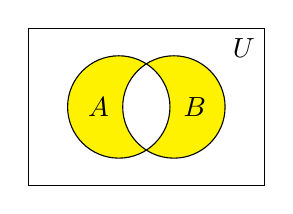
\begin{tikzpicture}
    \draw (0,0) --(0,2) --(3,2) --(3,0) --(0,0);
    \def\firstcircle{(1.15,1) circle [radius = 0.65]}
    \def\secondcircle{(1.85, 1) circle [radius = 0.65]}
    \node [left] at (3,1.75){\(U\)};

    \fill [even odd rule, yellow] \firstcircle \secondcircle;
    \draw \firstcircle \secondcircle;
    \node [left] at (1.15,1){\(A\)};
    \node [right] at (1.85, 1){\(B\)};
    \end{tikzpicture}
\end{center}

\newpage
\subsection{Properties}
\paragraph{Inclusion-Exclusion Principle}
The inclusion-exclusion principle helps to calculate the cardinality of unions of sets. The principle states that the cardinality of the union of \(A\) and \(B\) is equal to the cardinality of \(A\) plus the cardinality of \(B\) minus the cardinality of the intersection of \(A\) and \(B\).
\[ |A\cup B| = |A| + |B| - |A\cap B| \]

\begin{multicols}{2}
    \subparagraph{De Morgan's Laws}
    \[ \overline{A\cup B} = \bar{A}\cap\bar{B} \]
    \[ \overline{A\cap B} = \bar{A}\cup\bar{B} \]

    \subparagraph{Identity Laws}
    \[ A\cup\varnothing = A \]
    \[ A\cap U = A \]

    \subparagraph{Domination Laws}
    \[ A\cup U = U \]
    \[ A\cap\varnothing = \varnothing \]

    \subparagraph{Idempotent Laws}
    \[ A\cup A = A \]
    \[ A\cap A = A \]

    \subparagraph{Commutative Laws}
    \[ A\cup B = B\cup A \]
    \[ A\cap B = B\cap A \]

    \subparagraph{Associative Laws}
    \[ A\cup(B\cup C) = (A\cup B)\cup C \]
    \[ A\cap(B\cap C) = (A\cap B)\cap C \]

    \subparagraph{Distributive Laws}
    \[ A\cup(B\cap C) = (A\cup B)\cap (A\cup C) \]
    \[ A\cap(B\cup C) = (A\cap B)\cup (A\cap C) \]

    \subparagraph{Absorption Laws}
    \[ A\cup(A\cap B) = A \]
    \[ A\cap(A\cup B) = A \]

    \subparagraph{Complement Laws}
    \[ A\cup\bar{A} = U \]
    \[ A\cap\bar{A} = \varnothing \]

    \subparagraph{Double Negation Law}
    \[ \overline{\left(\bar{A}\right)} = A \]
\end{multicols}

\newpage
\section{Relations}
\subsection{Definitions}
A relation is the subset of the cartesian product of a number of sets. The simplest relation is a binary relation such as \(R\) from the set \(A\) to the set \(B\).
\[ R\subseteq A\times B \]
Given are the following sets \(A\) and \(B\) and the relation \(R\) from \(A\) to \(B\).
\[ A = \{a,b\}, B = \{0,1,2\}, R = \{(a,0),(a,2),(b,1),(b,2)\} \]
This relation can be visualised in the following ways.
\begin{multicols}{2}
\begin{center}
\begin{tabular}{c | c c}
    \(R\) & \(a\) & \(b\) \\
    \hline
    \(0\) & X &   \\
    \(1\) &   & X \\
    \(2\) & X & X \\
\end{tabular}
\end{center}
\begin{center}
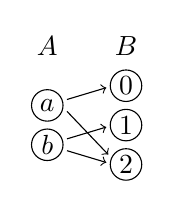
\begin{tikzpicture}[scale=0.5]
    \def\circleOne{(1,3.5) circle [radius=0.4]}
    \def\circleTwo{(1,2.5) circle [radius=0.4]}
    \def\circleThree{(3,4) circle [radius=0.4]}
    \def\circleFour{(3,3) circle [radius=0.4]}
    \def\circleFive{(3,2) circle [radius=0.4]}
    \draw \circleOne \circleTwo \circleThree \circleFour \circleFive;
    \node at (1,5){\(A\)};
    \node at (3,5){\(B\)};

    \node at (1,3.5){\(a\)};
    \node at (1, 2.5){\(b\)};

    \node at (3,4){\(0\)};
    \node at (3,3){\(1\)};
    \node at (3,2){\(2\)};

    \draw [->] (1.5,3.65) --(2.5,3.95);
    \draw [->] (1.5,3.35) --(2.55,2.25);
    \draw [->] (1.5,2.65) --(2.5,2.95);
    \draw [->] (1.5,2.35) --(2.5,2.05);
\end{tikzpicture}
\end{center}
\end{multicols}
\noindent
The following notation can be used to simply show whether or not the pair \((a,b)\) is in \(R\).
\[ a\mathrel{R}b = (a,b)\in R \]
\[ a\not\mathrel{R}b = (a,b)\notin R \]
The number of relations on a set \(A\) is equal to \(2\) to the power of of the cardinality of its cartesian product.
\[ 2^{|A\times A|} = 2^{|A|^2} \]
\subsection{Properties}
Relations are sets so the regular set operations can be used on them. Additionally it is possible to create a composition of two relations. If \(R_1\) is a relation from \(A\) to \(B\) and \(R_2\) is relation from \(B\) to \(C\) then \(R_2\circ R_1\) is a relation from \(A\) to \(C\).
\paragraph{Power of a relation}
\[ R^n = \left\{
\begin{array}{lr}
    R, & \text{for } n=1 \\
    R^{n-1}\circ R, & \text{for } n>1 \\
\end{array}
\right\}
\]
\subsubsection{Reflexivity}
A relation is reflexive if every element is related to itself.
\[ \forall a[a\in U\rightarrow (a,a)\in R] \]
This property can be seen in a matrix if there is a diagonal line through the matrix.
\begin{center}
    \begin{tabular}{c | c c c}
        \(R\) & \(a\) & \(b\) & \(c\) \\
        \hline
        \(a\) & \(1\) &       &       \\
        \(b\) &       & \(1\) &       \\
        \(c\) &       &       & \(1\) \\
    \end{tabular}
\end{center}
If this property is negated then a relation is irreflexive.
\subsubsection{Symmetry}
In a symmetric relation for every pair \((a,b)\) in \(R\) there must also be a pair \(b,a\).
\[ \forall a\forall b[(a,b)\in R \rightarrow (b,a)\in R] \]
The resulting matrix will also be a symmetric matrix.
\begin{center}
    \begin{tabular}{c | c c c}
        \(R\) & \(a\) & \(b\) & \(c\) \\
        \hline
        \(a\) & \(0\) & \(1\) & \(0\) \\
        \(b\) & \(1\) & \(0\) & \(1\) \\
        \(c\) & \(0\) & \(1\) & \(0\) \\
    \end{tabular}
\end{center}
In an anti-symmetric relation for every pair which has a symmetric counterpart the elements must be related to themselves.
\[ \forall a\forall y[(a,b)\in R \land (b,a)\in R \rightarrow x=y] \]
\subsubsection{Transitivity}
In a transitive relation if \((a,b)\in R\) and \((b,c \in R\) then \(a,c\in R\) must also be true.
\[ \forall a\forall b\forall c[(a,b)\in R\land (b,c)\in R\rightarrow (a,c)\in R] \]

\subsection{Representing Relations}
\subsection{Closures}
\subsection{Equivalence Relations}
\subsection{Equivalence Classes and Partitions}
\subsection{Comparability}

\subsection{Functions}
A special kind of relation is a function. A function is a subset of \(A\times B\) with the restriction that no two elements may have the same first element.
\[ \forall x\left[x\in A\rightarrow \exists y\left(y\in B\land (x,y)\in f\right)\right] \land \forall x,y_1,y_2\left[\left((x,y_1)\in f\land(x,y_2)\in f\right)\rightarrow y_1 = y_2 \right] \]
\subsubsection{Definitions}
A function is a mapping from one set to another. \(A\) and \(B\) are two non-empty sets and the function \(f\) is a mapping from \(A\) to \(B\).
\[f:A\rightarrow B\]
Each element of \(A\) is assigned to exactly to exactly one element \(B\).
\[f(a) = b\]
In this case the set \(A\) is the domain of the function and the set \(B\) is the co-domain. The range is a subset of the co-domain and contains all the elements of \(B\) that \(f\) actually maps to.

\begin{center}
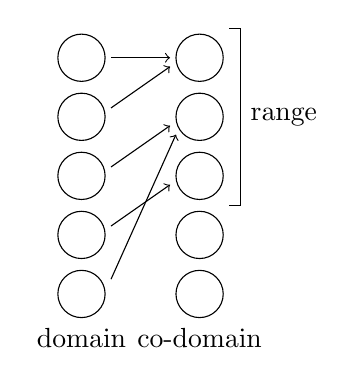
\begin{tikzpicture}[scale=0.75]
    \def\circleOne{(1,1) circle [radius=0.4]}
    \def\circleTwo{(1,2) circle [radius=0.4]}
    \def\circleThree{(1,3) circle [radius=0.4]}
    \def\circleFour{(1,4) circle [radius=0.4]}
    \def\circleFive{(1,5) circle [radius=0.4]}
    \def\circleSix{(3,1) circle [radius=0.4]}
    \def\circleSeven{(3,2) circle [radius=0.4]}
    \def\circleEight{(3,3) circle [radius=0.4]}
    \def\circleNine{(3,4) circle [radius=0.4]}
    \def\circleTen{(3,5) circle [radius=0.4]}
    \draw \circleOne \circleTwo \circleThree \circleFour \circleFive \circleSix \circleSeven \circleEight \circleNine \circleTen;
    \node at (1,0.25){domain};
    \node at (3,0.25){co-domain};
    \draw [->] (1.5,5) --(2.5,5);
    \draw [->] (1.5,4.15) --(2.5,4.85);
    \draw [->] (1.5,3.15) --(2.5,3.85);
    \draw [->] (1.5,2.15) --(2.5,2.85);
    \draw [->] (1.5,1.25) --(2.6,3.7);
    \draw (3.5,5.5) --(3.7,5.5) --(3.7,2.5) --(3.5,2.5);
    \node [right] at (3.7, 4){range};
\end{tikzpicture}
\end{center}

\subsubsection{Properties}
\paragraph{Addition \& Multiplication}
\[ (f_1 + f_2)(x) = f_1(x) + f_2(x) \]
\[ (f_1 f_2)(x) = f_1(x) f_2(x) \]
\paragraph{Increasing \& Decreasing}
\subparagraph{Increasing}
\[ \forall a,b\in A\left(a<b\rightarrow f(a)\leq f(b)\right) \]
\subparagraph{Strictly Increasing}
\[ \forall a,b\in A\left(a<b\rightarrow f(a)< f(b)\right) \]
\subparagraph{Decreasing}
\[ \forall a,b\in A\left(a<b\rightarrow f(a)\geq f(b)\right) \]
\subparagraph{Strictly Decreasing}
\[ \forall a,b\in A\left(a<b\rightarrow f(a)> f(b)\right) \]

\subsubsection{Types of Functions}
\paragraph{Injection}
Functions that are injective have a one-to-one mapping from \(A\) to \(B\). That means that every \(a\) is assigned to one \(b\) and every \(b\) is the image of at most one pre-image \(a\).
\[ \forall a,b(f(a)=f(b)\rightarrow a=b) \]
\begin{center}
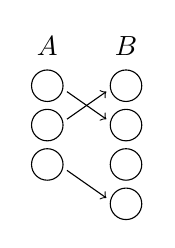
\begin{tikzpicture}[scale=0.5]
    \def\circleTwo{(1,2) circle [radius=0.4]}
    \def\circleThree{(1,3) circle [radius=0.4]}
    \def\circleFour{(1,4) circle [radius=0.4]}
    \def\circleSix{(3,1) circle [radius=0.4]}
    \def\circleSeven{(3,2) circle [radius=0.4]}
    \def\circleEight{(3,3) circle [radius=0.4]}
    \def\circleNine{(3,4) circle [radius=0.4]}
    \draw \circleTwo \circleThree \circleFour \circleSix \circleSeven \circleEight \circleNine;
    \node at (1,5){\(A\)};
    \node at (3,5){\(B\)};
    \draw [->] (1.5,3.85) --(2.5,3.15);
    \draw [->] (1.5,3.15) --(2.5,3.85);
    \draw [->] (1.5,1.85) --(2.5,1.15);
\end{tikzpicture}
\end{center}

\paragraph{Surjection}
A surjective function maps \(A\) onto \(B\), which means that for every element in \(B\) has a pre-image.
\[ \forall b\in B\left[\exists a\in A(f(a) = b)\right] \]
\begin{center}
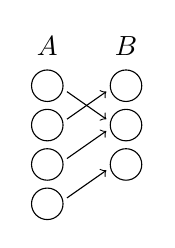
\begin{tikzpicture}[scale=0.5]
    \def\circleTwo{(1,2) circle [radius=0.4]}
    \def\circleThree{(1,3) circle [radius=0.4]}
    \def\circleFour{(1,4) circle [radius=0.4]}
    \def\circleSix{(1,1) circle [radius=0.4]}
    \def\circleSeven{(3,2) circle [radius=0.4]}
    \def\circleEight{(3,3) circle [radius=0.4]}
    \def\circleNine{(3,4) circle [radius=0.4]}
    \draw \circleTwo \circleThree \circleFour \circleSix \circleSeven \circleEight \circleNine;
    \node at (1,5){\(A\)};
    \node at (3,5){\(B\)};
    \draw [->] (1.5,3.85) --(2.5,3.15);
    \draw [->] (1.5,3.15) --(2.5,3.85);
    \draw [->] (1.5,2.15) --(2.5,2.85);
    \draw [->] (1.5,1.15) --(2.5,1.85);
\end{tikzpicture}
\end{center}

\paragraph{Bijection}
A bijection is a function, which is both injective and surjective.
\begin{center}
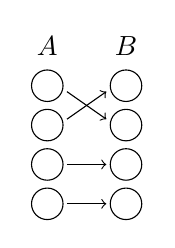
\begin{tikzpicture}[scale=0.5]
    \def\circleTwo{(1,2) circle [radius=0.4]}
    \def\circleThree{(1,3) circle [radius=0.4]}
    \def\circleFour{(1,4) circle [radius=0.4]}
    \def\circleFive{(1,1) circle [radius=0.4]}
    \def\circleSix{(3,1) circle [radius=0.4]}
    \def\circleSeven{(3,2) circle [radius=0.4]}
    \def\circleEight{(3,3) circle [radius=0.4]}
    \def\circleNine{(3,4) circle [radius=0.4]}
    \draw \circleTwo \circleThree \circleFour \circleFive \circleSix \circleSeven \circleEight \circleNine;
    \node at (1,5){\(A\)};
    \node at (3,5){\(B\)};
    \draw [->] (1.5,3.85) --(2.5,3.15);
    \draw [->] (1.5,3.15) --(2.5,3.85);
    \draw [->] (1.5,2) --(2.5,2);
    \draw [->] (1.5,1) --(2.5,1);
\end{tikzpicture}
\end{center}

\subsubsection{Inverse Function}
If the function \(f\) is bijective then it has an inverse. The inverse of \(f\) is denoted as \(f^{-1}\).

\begin{center}
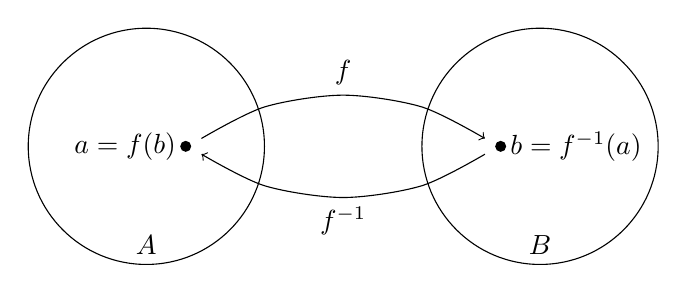
\begin{tikzpicture}
    \def\circleA{(1.5,2) circle [radius=1.5]}
    \def\circleB{(6.5,2) circle [radius=1.5]}
    \def\elementA{(2,2) circle [radius=0.07]}
    \def\elementB{(6,2) circle [radius=0.07]}
    \draw \circleA \circleB;
    \node [above] at (1.5, 0.5){\(A\)};
    \node [above] at (6.5, 0.5){\(B\)};

    \fill \elementA \elementB;
    \node [left] at (2,2){\(a=f(b)\)};  \node [right] at (6,2){\(b=f^{-1}(a)\)};

    \draw [->] plot [smooth] coordinates {(2.2,2.1) (3,2.5) (4,2.65) (5,2.5) (5.8,2.1)};
    \draw [->] plot [smooth] coordinates {(5.8,1.9) (5,1.5) (4,1.35) (3,1.5)(2.2,1.9)};

    \node [above] at (4,2.65){\(f\)};
    \node [below] at (4,1.35){\(f^{-1}\)};
\end{tikzpicture}
\end{center}

\subsubsection{Composition}
Given the functions \(f:B\rightarrow C\) and \(g:A\rightarrow B\), the composition \(f\circ g\) is the function \(A\rightarrow C\).
\[ f\circ g(x) = f\left(g(x)\right)\]

\begin{center}
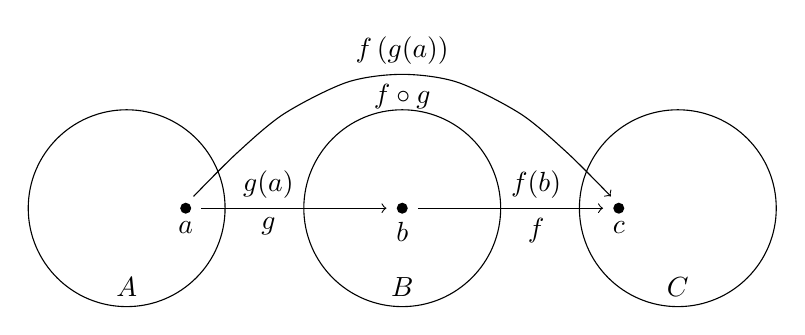
\begin{tikzpicture}
    \def\circleA{(1.5, 1.5) circle [radius=1.25]}
    \def\circleB{(5, 1.5) circle [radius=1.25]}
    \def\circleC{(8.5, 1.5) circle [radius=1.25]}
    \draw \circleA \circleB \circleC;
    \node [above] at (1.5, 0.25){\(A\)};
    \node [above] at (5, 0.25){\(B\)};
    \node [above] at (8.5, 0.25){\(C\)};
    \def\elementA{(2.25, 1.5) circle [radius=0.07]}
    \def\elementB{(5, 1.5) circle [radius=0.07]}
    \def\elementC{(7.75, 1.5) circle [radius=0.07]}
    \fill \elementA \elementB \elementC;
    \node [below] at (2.25, 1.45){\(a\)};
    \node [below] at (5, 1.45){\(b\)};
    \node [below] at (7.75, 1.45){\(c\)};

    \draw [->] (2.45, 1.5) --(4.8, 1.5);
    \node [below] at (3.3, 1.5){\(g\)};
    \node [above] at (3.3, 1.5){\(g(a)\)};

    \draw [->] (5.2, 1.5) --(7.55, 1.5);
    \node [below] at (6.7, 1.5){\(f\)};
    \node [above] at (6.7, 1.5){\(f(b)\)};

    \draw [->] plot [smooth] coordinates {(2.35, 1.65) (2.9, 2.2) (3.5, 2.7) (4.3,3.1) (5, 3.2) (5.7,3.1) (6.5, 2.7) (7.1, 2.2) (7.65, 1.65)};
    \node [below] at (5, 3.2){\(f\circ g\)};
    \node [above] at (5, 3.2){\(f\left(g(a)\right)\)};
\end{tikzpicture}
\end{center}
\subsection{Relational Alegebra}

\section{Graphs}

\subsection{Trees}

\end{document}
